\section{Experiments}

\subsection{Training Dataset}
To support robust tool learning through RL, we construct a mixed dataset spanning diverse tool use scenarios:

\begin{itemize}[topsep=2pt, leftmargin=10pt, itemsep=-2pt]
\item \textbf{ToolACE}~\citep{liu2024toolace}: A general tool use dataset where the model learns when to invoke tools versus respond directly, improving decision-making in multi-step interactions.

\item \textbf{Hammer (Masked)}~\citep{lin2024hammer}: A subset of Hammer with randomized tool and parameter names, forcing the model to rely on descriptions rather than memorized labels, thus enhancing generalization and reducing overfitting to certain tools.

\item \textbf{xLAM}~\citep{zhang2024xlam}: A compositional dataset requiring one or multiple tool calls per turn, encouraging the model to reason about tool dependencies and plan diverse tool calling action actively.
\end{itemize}

For RL training, we sample 2K examples from ToolACE and 1K each from Hammer and xLAM, creating a balanced dataset spanning diverse levels of complexity and tool use. Multi-step trajectories are decomposed into single-step instances, with prior dialogue history injected into the user prompt (as shown in \Cref{prompt:user}) to preserve context. This setup encourages strategic exploration and teaches the model to select and apply tools appropriately within each step. Please see \Cref{apdx:training} for more details and justifications.
% \xiusi{Is there a specific reason for sampling the data? Why not use the full training data?} \cheng{full data is too much is all data are of same distribution, we will explain in appendix}

\subsection{Experiment Settings}
\paragraph{Training.}  We conduct all RL experiments using the veRL framework~\citep{sheng2024hybridflow}, adopting the GRPO algorithm detailed in the previous section. For each training step, we sample a batch of 512, and generate 4 responses per query, training for 15 epochs in total (see \Cref{apdx:training} for full configuration details). To encourage broader policy exploration, we remove KL regularization and apply a generation temperature of 1.0. We initialize our models with the Qwen-2.5-Instruct~\citep{2024qwen2.5} and Llama-3.2-Instruct~\citep{dubey2024llama} series, which are further tuned under the GRPO objective with our customized reward design.

\paragraph{Evaluation.} We evaluate our approach on the \textbf{Berkeley Function Call Leaderboard} (BFCL)~\citep{patil2024gorilla}, a comprehensive benchmark that spans a diverse set of challenges, including single-step reasoning, multi-step tool use, real-time execution, irrelevant tool rejection, simultaneous multi-tool selection, and multi-tool application\footnote{\url{https://gorilla.cs.berkeley.edu/blogs/13_bfcl_v3_multi_turn.html}}. In addition, we present results on \textbf{API-Bank}~\citep{li2023api}, a three-level evaluation framework comprising 73 diverse and complex API tools. It assesses an LLM’s ability to select and apply tools through natural multi-turn dialogues, across three levels of difficulty. We also evaluate on a representative QA benchmark \textbf{Bamboogle}~\citep{press2022measuring}, which comprises a variety of question-answering tasks where performance is measured based on the final answer accuracy rather than the correctness of tool use. These broad coverage makes our evaluation setting effective for evaluating real-world LLM tool use proficiency. All results are reported in terms of accuracy.
% \emre{bamboogle?}\cheng{Make bamboogle an additional study here, we could change later in submission version}

\paragraph{Baselines.} We compare our approach against several baselines to better isolate the effects of GRPO training: (1) \textbf{Raw Instruct Model}: the original model without any additional fine-tuning or RL, evaluated using the same prompts. (2) \textbf{SFT on RL Data}: the instruct model fine-tuned using the same 4K / selected 400 data points as the RL training set, providing a comparison point to assess whether GRPO training outperforms standard SFT. (3) \textbf{GRPO on SFT Model}: GRPO is applied to a model that has already undergone SFT on the selected 400 data points. This setup allows us to evaluate the impact of initializing GRPO with a format-aware model, in contrast to starting from the raw instruct model in a cold start manner. (4) \textbf{PPO:} We also include the standard PPO setting as a baseline to evaluate whether our reward design is effective beyond GRPO. We report results for both a cold start PPO model and a PPO model initialized with SFT, using the same hyperparameters as in the GRPO setup for a fair comparison. Please refer to \Cref{apdx:training} for more details and justifications.

% \emre{we should decide which one to show, my bet is for 4k}
% \emre{maybe we say I/O prompting baseline}
% \hongru{the baseline here is a little weird, why bother to have another 400 data points (and how to select them?) and why not adding SFT4k + GRPO?} \cheng{because this 4k data is also used for GRPO, this setting entails SFT and RL done with the same data which is also kind of weird. Current 400 data is not in 4k, but of the same distribution and randomly selected} \hongru{My point is you need to explain why you need this sft 400 data and why 400 instead of 300. Basically I do not see the motivation about this, and sft4k + GRPO can show the upper bound or show the power of sft on same data.} \cheng{more explained in appendix}


\subsection{Results}

\begin{table*}[!t]
\centering
\resizebox{1.0\linewidth}{!}{
\begin{tabular}{lccccccc}
\toprule
\textbf{Model} & \textbf{Overall Acc} & Non-Live AST Acc & Non-Live Exec Acc & Live Acc & Multi Turn Acc & Relevance Detection & Irrelevance Detection \\
\midrule
Qwen2.5-1.5B-Instruct (\textbf{Raw}) & 19.41\% & 16.00\% & 13.18\% & 35.58\% & 0.00\% & 44.44\% & 82.49\% \\
Qwen2.5-1.5B-Instruct (\textbf{SFT400}) & 40.21\% & 65.12\% & 61.11\% & 56.69\% & 1.00\% & 94.44\% & 60.14\% \\
Qwen2.5-1.5B-Instruct (\textbf{SFT4k}) & 40.67\% & 59.94\% & 59.84\% & 59.31\% & 1.00\% & 88.89\% & 71.34\% \\
Qwen2.5-1.5B-Instruct (\textbf{SFT400+PPO}) & \uline{42.95\%} & 77.65\% & 69.75\% & 55.73\% & 1.88\% & 100.00\% & 48.40\% \\
Qwen2.5-1.5B-Instruct (\textbf{SFT400+GRPO}) & 40.93\% & 70.54\% & 60.79\% & 56.33\% & 1.00\% & 94.44\% & 58.63\% \\
% Qwen2.5-1.5B-Instruct (\textbf{SFT4k+PPO}) & 40.24\% & 66.42\% & 62.02\% & 54.58\% & 2.50\% & 94.12\% & 55.09\% \\
% Qwen2.5-1.5B-Instruct (\textbf{SFT4k+GRPO}) & \uline{42.63\%} & 66.60\% & 64.77\% & 60.15\% & 1.38\% & 88.89\% & 67.98\% \\
Qwen2.5-1.5B-Instruct (\textbf{PPO Cold Start}) & 38.32\% & 79.40\% & 70.11\% & 45.24\% & 0.87\% & 100.00\% & 18.09\% \\
Qwen2.5-1.5B-Instruct (\textbf{Ours, GRPO Cold Start}) & \textbf{46.20\%} & 77.96\% & 76.98\% & 60.73\% & 2.25\% & 100.00\% & 56.44\% \\
\midrule
Qwen2.5-3B-Instruct (\textbf{Raw}) & 33.04\% & 42.52\% & 40.80\% & 53.96\% & 1.00\% & 64.71\% & 56.01\% \\
Qwen2.5-3B-Instruct (\textbf{SFT400}) & 34.08\% & 69.29\% & 61.50\% & 41.40\% & 0.00\% & 94.44\% & 8.11\% \\
Qwen2.5-3B-Instruct (\textbf{SFT4k}) & 41.97\% & 62.85\% & 54.73\% & 59.17\% & 0.75\% & 77.78\% & 75.12\% \\
Qwen2.5-3B-Instruct (\textbf{SFT400+PPO}) & 45.80\% & 78.29\% & 71.09\% & 58.76\% & 5.12\% & 94.12\% & 54.70\% \\
Qwen2.5-3B-Instruct (\textbf{SFT400+GRPO}) & 46.42\% & 76.21\% & 68.93\% & 64.15\% & 1.75\% & 88.89\% & 71.76\% \\
% Qwen2.5-3B-Instruct (\textbf{SFT4k+PPO}) & 48.22\% & 77.75\% & 73.18\% & 64.27\% & 5.25\% & 94.12\% & 66.41\% \\
% Qwen2.5-3B-Instruct (\textbf{SFT4k+GRPO}) & 47.82\% & 75.12\% & 69.52\% & 68.19\% & 2.38\% & 77.78\% & 76.16\% \\
Qwen2.5-3B-Instruct (\textbf{PPO Cold Start}) & \uline{51.15\%} & 82.42\% & 78.52\% & 67.78\% & 4.88\% & 94.12\% & 73.87\% \\
Qwen2.5-3B-Instruct (\textbf{Ours, GRPO Cold Start}) & \textbf{52.98\%} & 81.58\% & 79.43\% & 73.78\% & 3.75\% & 88.24\% & 84.85\% \\
\midrule
Qwen2.5-7B-Instruct (\textbf{Raw}) & 41.97\% & 66.02\% & 70.11\% & 53.51\% & 4.25\% & 76.47\% & 62.66\% \\
Qwen2.5-7B-Instruct (\textbf{SFT400}) & 34.08\% & 69.29\% & 66.68\% & 41.4\% & 0.00\% & 94.44\% & 8.11\% \\
Qwen2.5-7B-Instruct (\textbf{SFT4k}) & 36.53\% & 45.15\% & 53.5\% & 57.13\% & 0.75\% & 72.22\% & 72.32\% \\
Qwen2.5-7B-Instruct (\textbf{SFT400+PPO}) & 42.02\% & 83.90\% & 72.62\% & 51.84\% & 0.25\% & 100.00\% & 29.66\% \\
Qwen2.5-7B-Instruct (\textbf{SFT400+GRPO}) & 39.25\% & 80.69\% & 74.34\% & 46.51\% & 0.25\% & 100.00\% & 14.19\% \\
% Qwen2.5-7B-Instruct (\textbf{SFT4k+PPO}) &  &  &  &  &  &  &  \\
% Qwen2.5-7B-Instruct (\textbf{SFT4k+GRPO}) & 35.18\% & 43.58\% & 50.39\% & 55.49\% & 0.87\% & 77.78\% & 67.12\% \\
Qwen2.5-7B-Instruct (\textbf{PPO Cold Start}) & \uline{46.68\%} & 79.33\% & 78.16\% & 63.17\% & 0.38\% & 88.89\% & 52.92\% \\
Qwen2.5-7B-Instruct (\textbf{Ours, GRPO Cold Start}) & \textbf{58.38\%} & 86.17\% & 78.25\% & 74.9\% & 18.12\% & 83.33\% & 76.68\%  \\
\midrule
Llama-3.2-3B-Instruct (\textbf{Raw}) & 22.09\% & 17.44\% & 14.57\% & 43.85\% & 0.00\% & 77.78\% & 66.07\% \\
Llama-3.2-3B-Instruct (\textbf{SFT400}) & 41.22\% & 64.27\% & 62.18\% & 58.37\% & 0.75\% & 66.67\% & 71.12\% \\
Llama-3.2-3B-Instruct (\textbf{SFT4k}) & \textbf{44.16\%} & 65.42\% & 67.02\% & 63.04\% & 1.38\% & 77.78\% & 78.25\% \\
Llama-3.2-3B-Instruct (\textbf{SFT400+PPO}) & 41.62\% & 68.10\% & 69.88\% & 52.98\% & 3.00\% & 94.12\% & 56.29\% \\
Llama-3.2-3B-Instruct (\textbf{SFT400+GRPO}) & 42.54\% & 65.15\% & 68.98\% & 59.40\% & 0.88\% & 72.22\% & 65.80\% \\
% Llama-3.2-3B-Instruct (\textbf{SFT4k+PPO}) & 45.41\% & 73.71\% & 68.46\% & 62.27\% & 2.50\% & 82.35\% & 68.75\% \\
% Llama-3.2-3B-Instruct (\textbf{SFT4k+GRPO}) & \textbf{45.50\%} & 70.69\% & 67.70\% & 64.73\% & 1.00\% & 77.78\% & 78.85\% \\
Llama-3.2-3B-Instruct (\textbf{PPO Cold Start}) & 42.98\% & 84.00\% & 72.00\% & 52.80\% & 2.88\% & 100.00\% & 31.94\% \\
Llama-3.2-3B-Instruct (\textbf{Ours, GRPO Cold Start}) & \uline{44.10\%} & 74.38\% & 75.18\% & 56.86\% & 1.37\% & 94.44\% & 62.23\% \\
\bottomrule
\end{tabular}
}
\caption{BFCL V3 Benchmark Results (Main Result)}
\label{tab:bfcl-result-main}
\end{table*}

%%%%%%%%%%%%%%%%%%%%%%%%%%%%%%%%%%%%%%%%

\begin{table*}[!t]
\centering

\begin{minipage}[t]{0.51\linewidth}
\centering

\resizebox{1\linewidth}{!}{
\begin{tabular}{lcccc}
\toprule
\textbf{Model} & \textbf{Overall Acc} & Level 1 & Level 2 & Level 3 \\
\midrule
Qwen2.5-1.5B-Instruct (\textbf{Raw}) & 30.65\% & 28.32\% & 35.82\% & 35.11\% \\
Qwen2.5-1.5B-Instruct (\textbf{SFT400}) & 53.60\% & 57.14\% & 50.75\% & 44.27\% \\
Qwen2.5-1.5B-Instruct (\textbf{SFT4k}) & 47.07\% & 52.88\% & 52.24\% & 26.72\% \\
Qwen2.5-1.5B-Instruct (\textbf{SFT400+PPO}) & 57.12\% & 60.9\% & 50.75\% & 48.85\% \\
Qwen2.5-1.5B-Instruct (\textbf{SFT400+GRPO}) & \uline{61.31\%} & 64.16\% & 58.21\% & 54.20\% \\
% Qwen2.5-1.5B-Instruct (\textbf{SFT4k+PPO}) & 61.31\% & 64.91\% & 56.72\% & 52.67\% \\
% Qwen2.5-1.5B-Instruct (\textbf{SFT4k+GRPO}) & 59.46\% & 65.16\% & 53.73\% & 45.04\% \\
Qwen2.5-1.5B-Instruct (\textbf{PPO Cold Start}) & 40.54\% & 44.61\% & 31.34\% & 32.82\% \\
Qwen2.5-1.5B-Instruct (\textbf{Ours, GRPO Cold Start}) & \textbf{63.15}\% & 70.68\% & 61.19\% & 41.22\% \\
\midrule
Qwen2.5-3B-Instruct (\textbf{Raw}) & 51.59\% & 59.65\% & 32.84\% & 36.64\% \\
Qwen2.5-3B-Instruct (\textbf{SFT400}) & 52.76\% & 59.65\% & 50.75\% & 32.82\% \\
Qwen2.5-3B-Instruct (\textbf{SFT4k}) & 50.92\% & 55.64\% & 43.28\% & 40.46\% \\
Qwen2.5-3B-Instruct (\textbf{SFT400+PPO}) & \uline{65.16\%} & 67.92\% & 55.22\% & 61.83\% \\
Qwen2.5-3B-Instruct (\textbf{SFT400+GRPO}) & 62.48\% & 68.67\% & 58.21\% & 45.80\% \\
% Qwen2.5-3B-Instruct (\textbf{SFT4k+PPO}) & 60.13\% & 64.41\% & 44.78\% & 54.96\% \\
% Qwen2.5-3B-Instruct (\textbf{SFT4k+GRPO}) & 60.80\% & 64.41\% & 56.72\% & 51.91\% \\
Qwen2.5-3B-Instruct (\textbf{PPO Cold Start}) & 57.62\% & 64.66\% & 59.70\% & 35.11\% \\
Qwen2.5-3B-Instruct (\textbf{Ours, GRPO Cold Start}) & \textbf{67.00\%} & 73.43\% & 67.16\% & 47.33\% \\
\midrule
Qwen2.5-7B-Instruct (\textbf{Raw}) & 62.48\% & 70.68\% & 49.25\% & 44.27\% \\
Qwen2.5-7B-Instruct (\textbf{SFT400}) & 50.59\% & 55.89\% & 50.75\% & 34.35\% \\
Qwen2.5-7B-Instruct (\textbf{SFT4k}) & 47.07\% & 51.13\% & 34.33\%&41.22\% \\
Qwen2.5-7B-Instruct (\textbf{SFT400+PPO}) & \uline{63.15\%} & 72.43\% & 58.21\% & 37.40\% \\
Qwen2.5-7B-Instruct (\textbf{SFT400+GRPO}) & 54.10\% & 61.40\% & 52.24\% &32.82\% \\
% Qwen2.5-7B-Instruct (\textbf{SFT4k+PPO}) & 59.30\% & 61.40\% & 40.3\% & 61.6\% \\
% Qwen2.5-7B-Instruct (\textbf{SFT4k+GRPO}) & & & & \\
Qwen2.5-7B-Instruct (\textbf{PPO Cold Start}) & 61.64\% & 68.67\% & 44.78\% & 48.85\% \\
Qwen2.5-7B-Instruct (\textbf{Ours, GRPO Cold Start}) & \textbf{64.66\%} & 73.93\% & 61.19\% & 38.17\% \\
\midrule
Llama-3.2-3B-Instruct (\textbf{Raw}) & 40.54\% & 44.86\% & 29.85\% & 32.82\% \\
Llama-3.2-3B-Instruct (\textbf{SFT400}) & 52.76\% & 60.65\% & 35.82\% & 37.40\% \\
Llama-3.2-3B-Instruct (\textbf{SFT4k}) & 43.89\% & 53.88\% & 29.85\% & 20.61\% \\
Llama-3.2-3B-Instruct (\textbf{SFT400+PPO}) & 57.79\% & 63.16\% & 47.76\% & 46.56\% \\
Llama-3.2-3B-Instruct (\textbf{SFT400+GRPO}) & \uline{56.78\%} & 63.60\% & 41.79\% & 43.51\% \\
% Llama-3.2-3B-Instruct (\textbf{SFT4k+PPO}) & 54.10\% & 60.65\% & 40.30\% & 41.22\% \\
% Llama-3.2-3B-Instruct (\textbf{SFT4k+GRPO}) & 50.92\% & 59.15\% & 34.33\% & 34.35\% \\
Llama-3.2-3B-Instruct (\textbf{PPO Cold Start}) & 55.78\% & 60.65\% & 41.79\% & 48.09\% \\
Llama-3.2-3B-Instruct (\textbf{Ours, GRPO Cold Start}) & \textbf{59.13\%} & 65.66\% & 52.24\% & 42.75\% \\
\bottomrule
\end{tabular}
}
\caption{API-Bank Test Results (Main Result)}
\label{tab:apibank-result-main}

\end{minipage}
\hfill
\begin{minipage}[t]{0.452\textwidth}
\centering

\resizebox{1\linewidth}{!}{
\begin{tabular}{lcccc}
\toprule
\textbf{Model} & \textbf{Accuracy} & Avg Num Tool Call \\
\midrule
Qwen2.5-1.5B-Instruct (\textbf{Raw}) & 20.8\% & 0.61 \\
Qwen2.5-1.5B-Instruct (\textbf{SFT400}) & 24.8\% & 0.78 \\
Qwen2.5-1.5B-Instruct (\textbf{SFT4k}) & 23.2\% & 1.25 \\
Qwen2.5-1.5B-Instruct (\textbf{SFT400+PPO}) & 36.8\% & 1.06 \\
Qwen2.5-1.5B-Instruct (\textbf{SFT400+GRPO}) & \uline{38.4\%} & 0.96 \\
% Qwen2.5-1.5B-Instruct (\textbf{SFT4k+PPO}) & 36.8\% & 1.06 \\
% Qwen2.5-1.5B-Instruct (\textbf{SFT4k+GRPO}) & 34.4\% & 1.02 \\
Qwen2.5-1.5B-Instruct (\textbf{PPO Cold Start}) & 23.2\% & 2.38 \\
Qwen2.5-1.5B-Instruct (\textbf{Ours, GRPO Cold Start}) & \textbf{44.0\%} & 1.19 \\
\midrule
Qwen2.5-3B-Instruct (\textbf{Raw}) & 52.0\% & 1.77 \\
Qwen2.5-3B-Instruct (\textbf{SFT400}) & 54.4\% & 0.86 \\
Qwen2.5-3B-Instruct (\textbf{SFT4k}) & 49.6\% & 0.92 \\
Qwen2.5-3B-Instruct (\textbf{SFT400+PPO}) & 43.2\% & 1.04 \\
Qwen2.5-3B-Instruct (\textbf{SFT400+GRPO}) & \uline{56.8\%} & 0.99 \\
% Qwen2.5-3B-Instruct (\textbf{SFT4k+PPO}) & 46.4\% & 1.01 \\
% Qwen2.5-3B-Instruct (\textbf{SFT4k+GRPO}) & 47.2\% & 0.98 \\
Qwen2.5-3B-Instruct (\textbf{PPO Cold Start}) & 40.0\% & 1.14 \\
Qwen2.5-3B-Instruct (\textbf{Ours, GRPO Cold Start}) & \textbf{60.0\%} & 1.32 \\
\midrule
Qwen2.5-7B-Instruct (\textbf{Raw}) & \uline{69.6\%} & 1.42 \\
Qwen2.5-7B-Instruct (\textbf{SFT400}) & 28.8\% & 3.71 \\
Qwen2.5-7B-Instruct (\textbf{SFT4k}) &  30.4\% & 1.06 \\
Qwen2.5-7B-Instruct (\textbf{SFT400+PPO}) &  45.6\% & 3.54 \\
Qwen2.5-7B-Instruct (\textbf{SFT400+GRPO}) & 29.6\% & 3.70 \\
% Qwen2.5-7B-Instruct (\textbf{SFT4k+PPO}) & 40.0\% & 1.25 \\
% Qwen2.5-7B-Instruct (\textbf{SFT4k+GRPO}) & 32.0\% & 1.25 \\
Qwen2.5-7B-Instruct (\textbf{PPO Cold Start}) & 48.0\% & 1.25 \\
Qwen2.5-7B-Instruct (\textbf{Ours, GRPO Cold Start}) & \textbf{72.0\%} &  1.63\\
\midrule
Llama-3.2-3B-Instruct (\textbf{Raw}) & 34.4\% & 1.25 \\
Llama-3.2-3B-Instruct (\textbf{SFT400})  & 44.0\% & 0.98 \\
Llama-3.2-3B-Instruct (\textbf{SFT4k}) & \uline{48.8\%} & 0.98 \\
Llama-3.2-3B-Instruct (\textbf{SFT400+PPO}) & 39.2\% & 1.33 \\
Llama-3.2-3B-Instruct (\textbf{SFT400+GRPO}) & 45.6\% & 1.00 \\
% Llama-3.2-3B-Instruct (\textbf{SFT4k+PPO}) & 49.6\% & 1.02 \\
% Llama-3.2-3B-Instruct (\textbf{SFT4k+GRPO}) & 42.4\% & 1.03 \\
Llama-3.2-3B-Instruct (\textbf{PPO Cold Start}) & 29.6\% & 1.42 \\
Llama-3.2-3B-Instruct (\textbf{Ours, GRPO Cold Start}) & \textbf{52.0\%} & 0.89 \\
\bottomrule
\end{tabular}
}
\caption{Bamboogle Test Results (Main Result)}
% \caption{Testing GRPO and baseline models on multi-step tool use in QA task, evaluated on the held-out Bamboogle test set.}
\label{tab:bamboogle-result-main}

\end{minipage}

\end{table*}


\paragraph{Main Results.} We report BFCL and API-Bank results in \Cref{tab:bfcl-result-main} and \Cref{tab:apibank-result-main}, respectively. Our GRPO method, trained from scratch on the Qwen2.5-Instruct series, generally outperforms other baselines, achieving \~10\% absolute gains over SFT trained on the same data volume. In contrast, LLaMA-3.2-Instruct shows less improvement, possibly due to the model's lower adaptability to GRPO-style generalization. Nevertheless, it remains competitive and outperforms most baselines on API-Bank.
% \hongru{why sft400 better than sft4k in api-bank but worse on BFCL?} \cheng{Yes, it's kind of hard to predict SFT behavior on held-out tasks ... But empirical results indeed show as they are}

\begin{figure}
    \centering
    \subfigure[Format Reward]{
        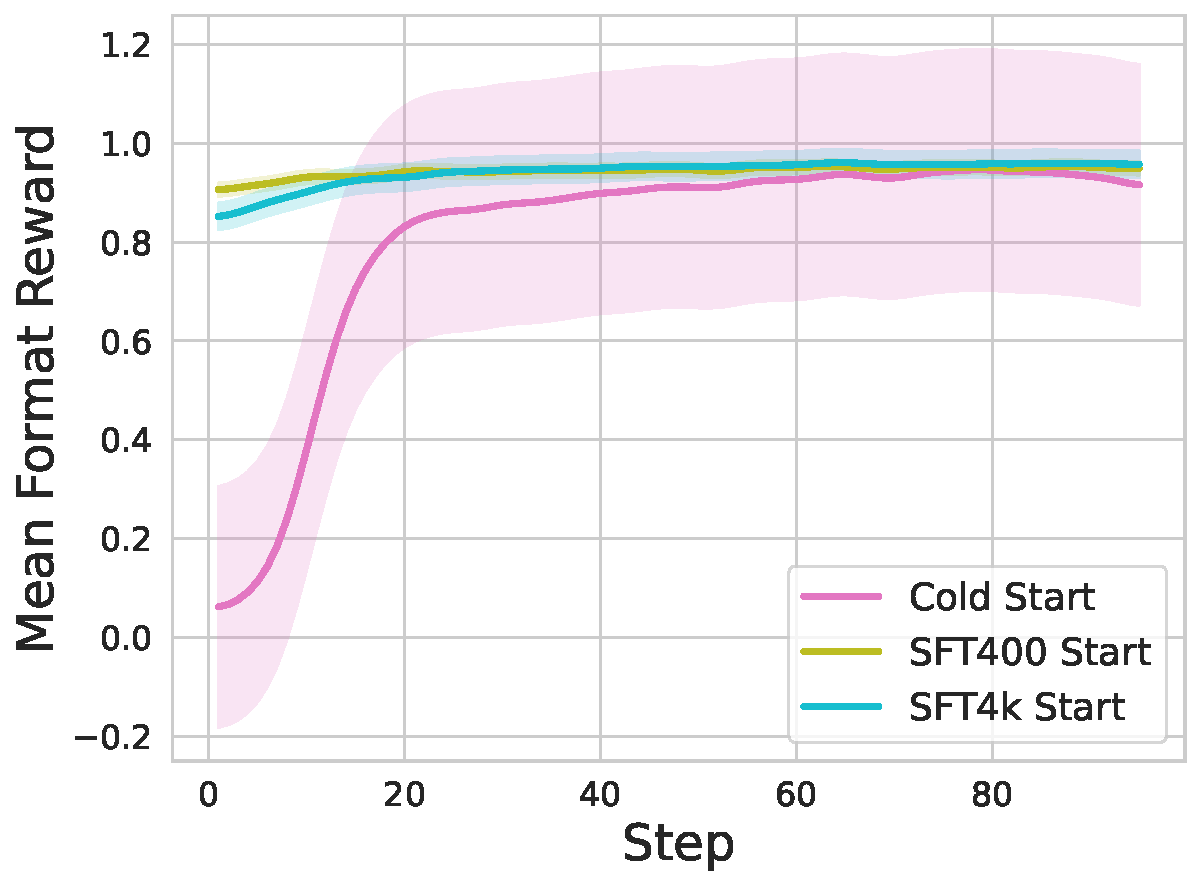
\includegraphics[width=0.469\linewidth]{figures/main_format.pdf}
    }
    \hfill
    \subfigure[Correctness Reward]{
        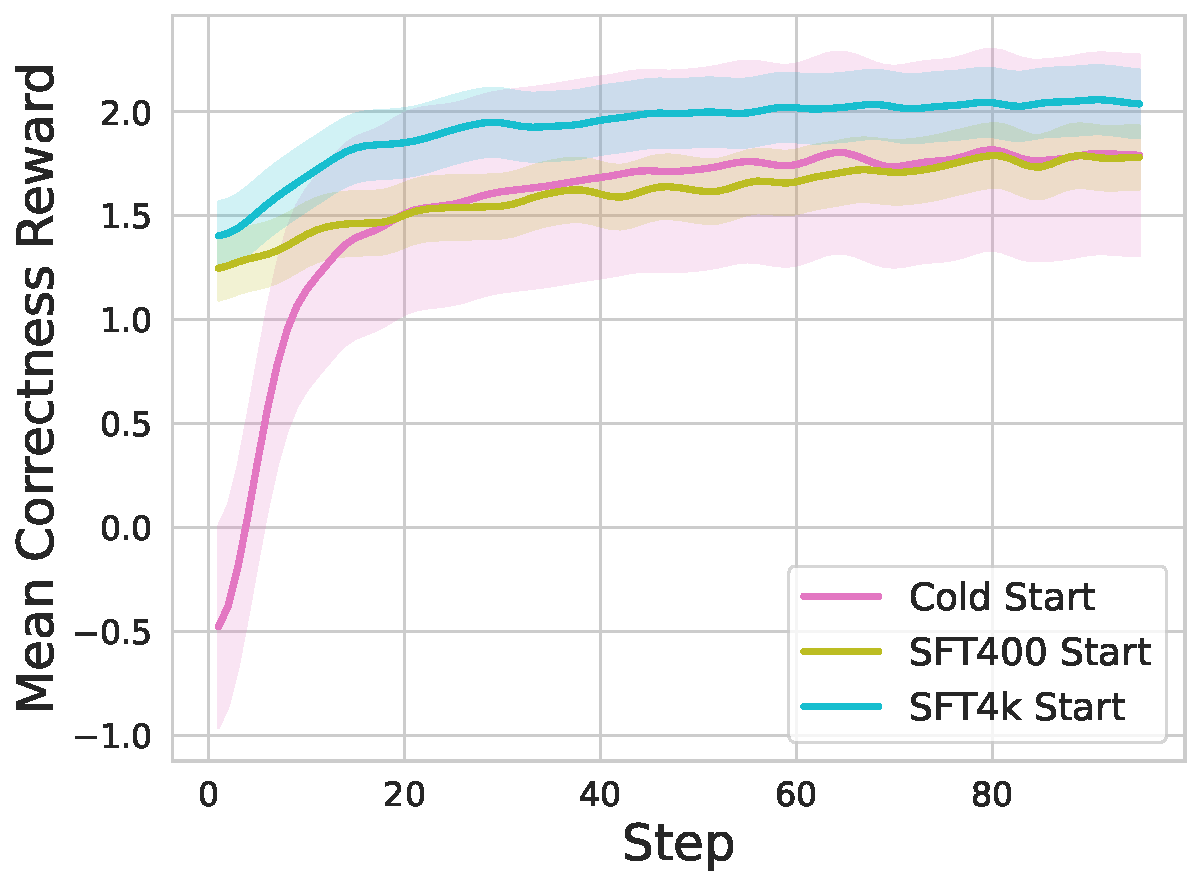
\includegraphics[width=0.469\linewidth]{figures/main_correctness.pdf}
    }
    \caption{Format (left) and correctness (right) reward trends across training steps for Qwen2.5-3B-Instruct with different model initialization strategies.}
    \label{fig:main_initialization}
\end{figure}


\paragraph{SFT Initialization Impacts.} Interestingly, GRPO also improves models initialized with limited SFT, often outperforming full-scale SFT trained on 10 times more data. However, this setup still underperforms compared to cold start GRPO. We hypothesize that SFT initialization leads to memorization and overfitting, which reduces the impact of GRPO’s effectiveness in generalization. As shown in \Cref{fig:main_initialization}, SFT-initialized models achieve higher training rewards due to distributional alignment between SFT and RL data, but empirically generalize worse on the two benchmarks. This further highlights that higher training rewards do not necessarily translate to better generalization.
% \hongru{do not see this result?}\cheng{all tested benchmarks are held-out tasks}

\begin{figure}
    \centering
    \subfigure[Format Reward]{
        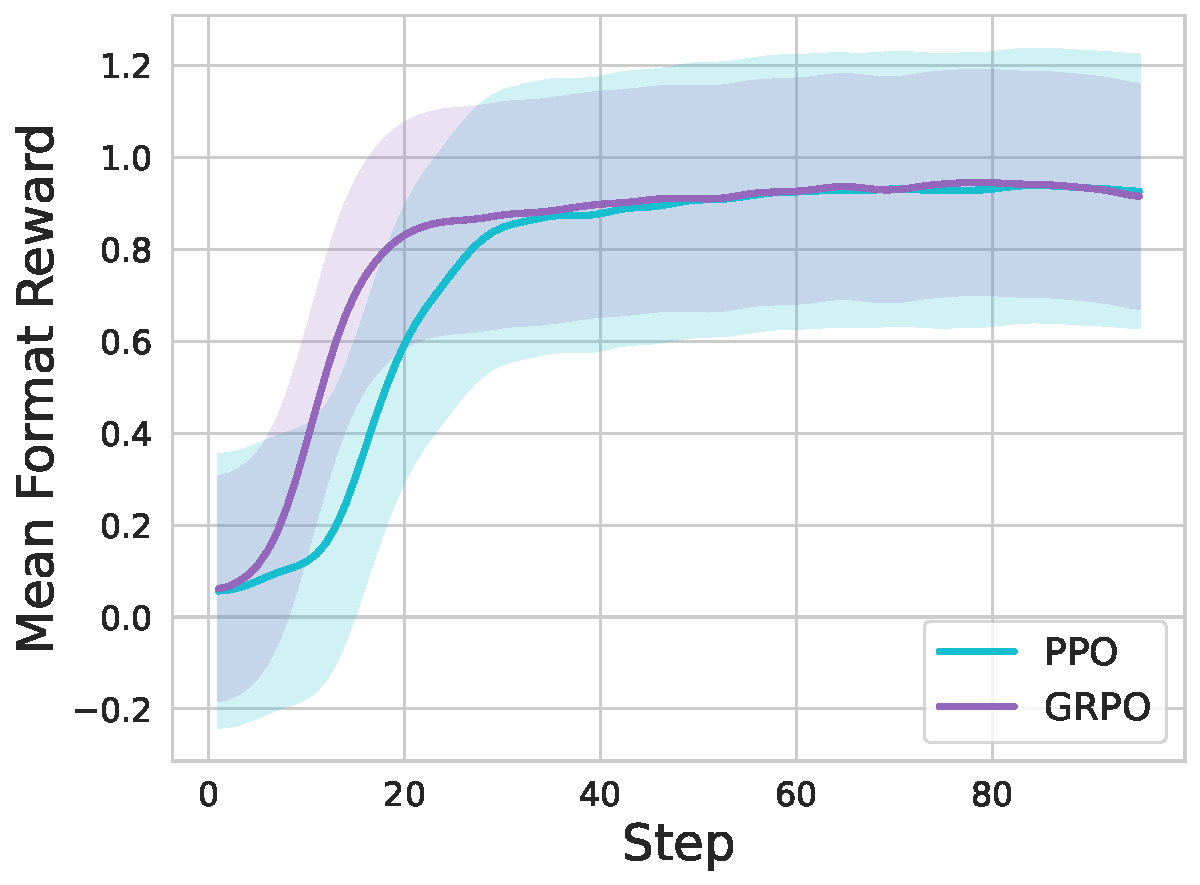
\includegraphics[width=0.469\linewidth]{figures/ppo_format.pdf}
    }
    \hfill
    \subfigure[Correctness Reward]{
        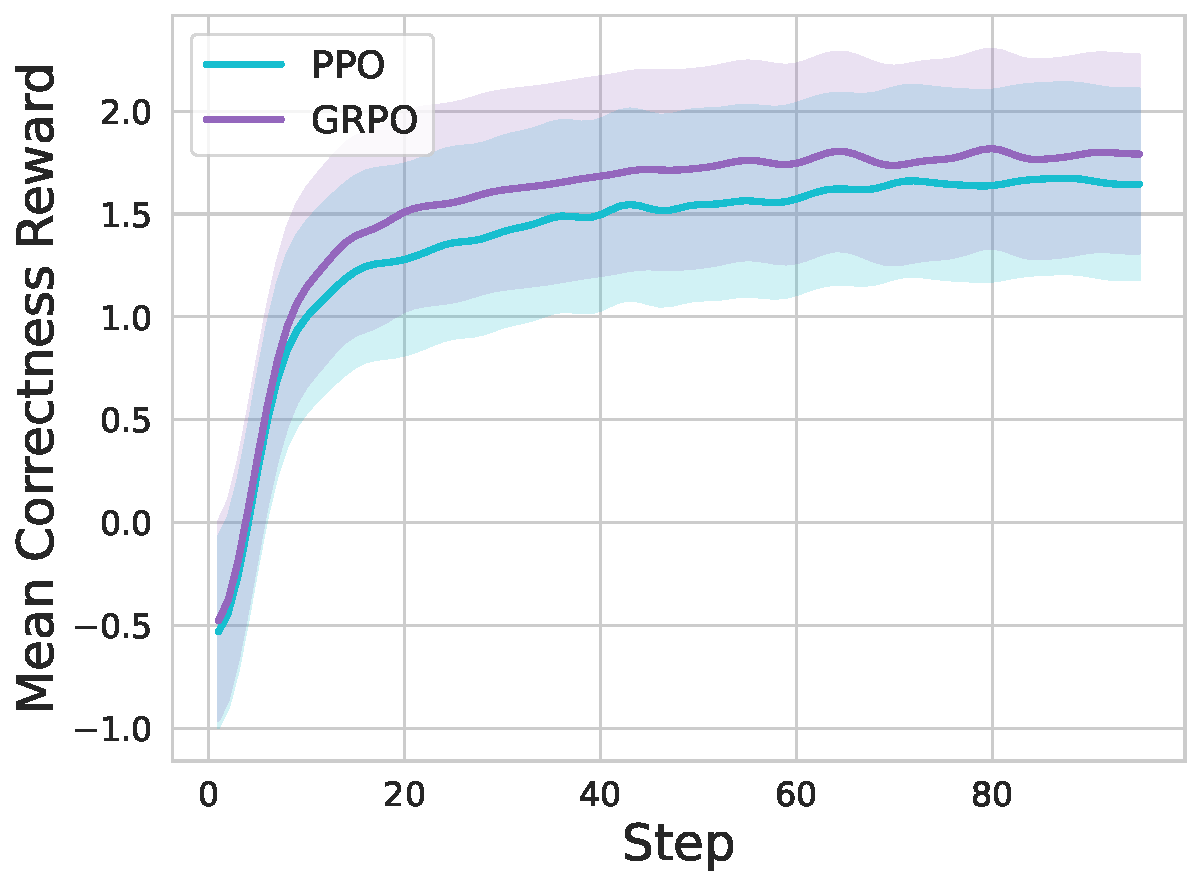
\includegraphics[width=0.469\linewidth]{figures/ppo_correctness.pdf}
    }
    \caption{Format (left) and correctness (right) reward trends across training steps for Qwen2.5-3B-Instruct with different RL strategies (GRPO v.s. PPO).}
    \label{fig:main_ppo}
\end{figure}

\paragraph{Reward Design on PPO.} We also evaluate PPO under both cold start and SFT-initialized settings to examine the effectiveness of our reward design. The results show that while PPO with a cold start can outperform SFT in some cases, it tends to be less stable across different model settings. In contrast, GRPO consistently achieves higher rewards even from a cold start, suggesting that our reward design is partially effective for PPO but works best in the GRPO framework. As shown in \Cref{fig:main_ppo}, GRPO not only achieves higher correctness rewards but also gains format rewards more rapidly during training. Interestingly, PPO benefits from SFT initialization, generally yielding better results than a cold start, whereas GRPO performs better when trained from scratch. These findings highlight that while PPO can benefit from our reward design, its impact is more limited compared to the more robust and consistent improvements observed with GRPO.


\begin{figure}
    \centering
    \subfigure[Unfamiliar Scenario]{
        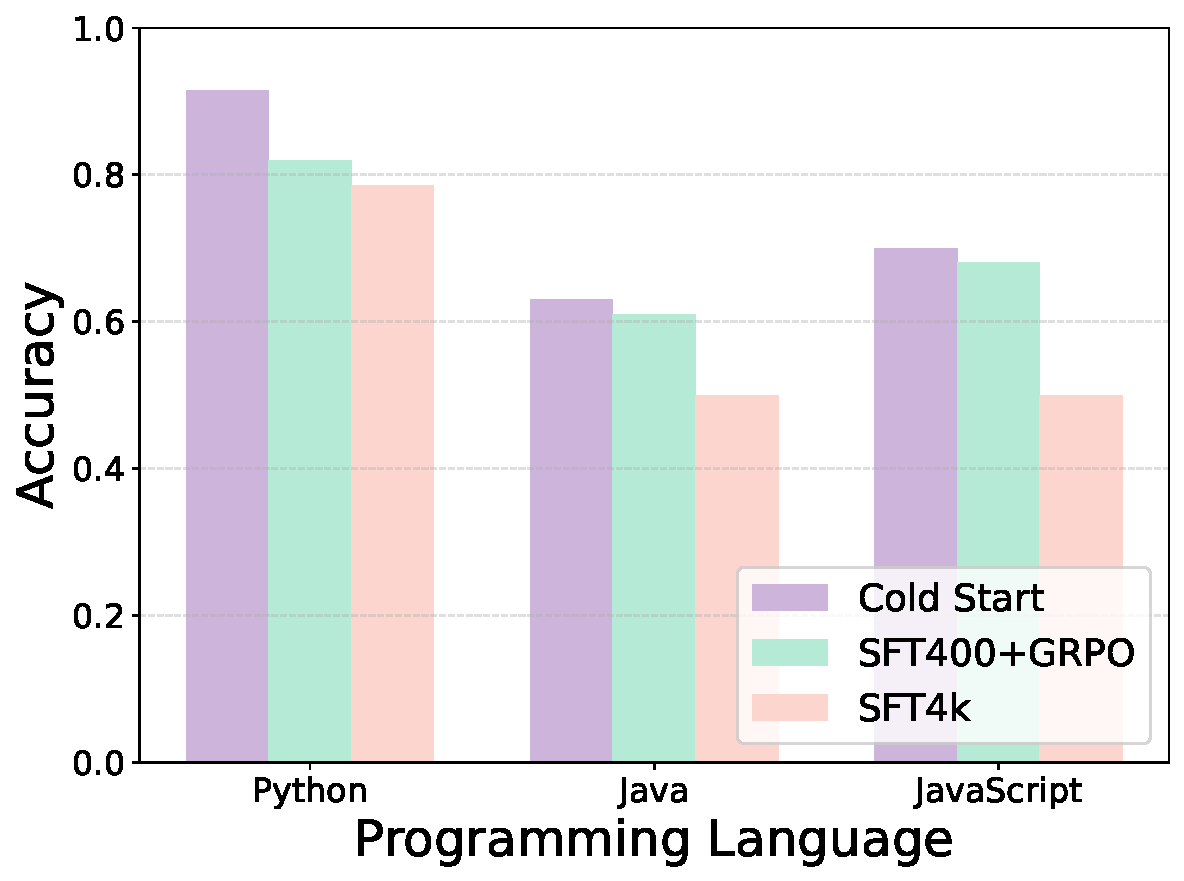
\includegraphics[width=0.469\linewidth]{figures/main_setting.pdf}
    }
    \hfill
    \subfigure[Unfamiliar Goal]{
        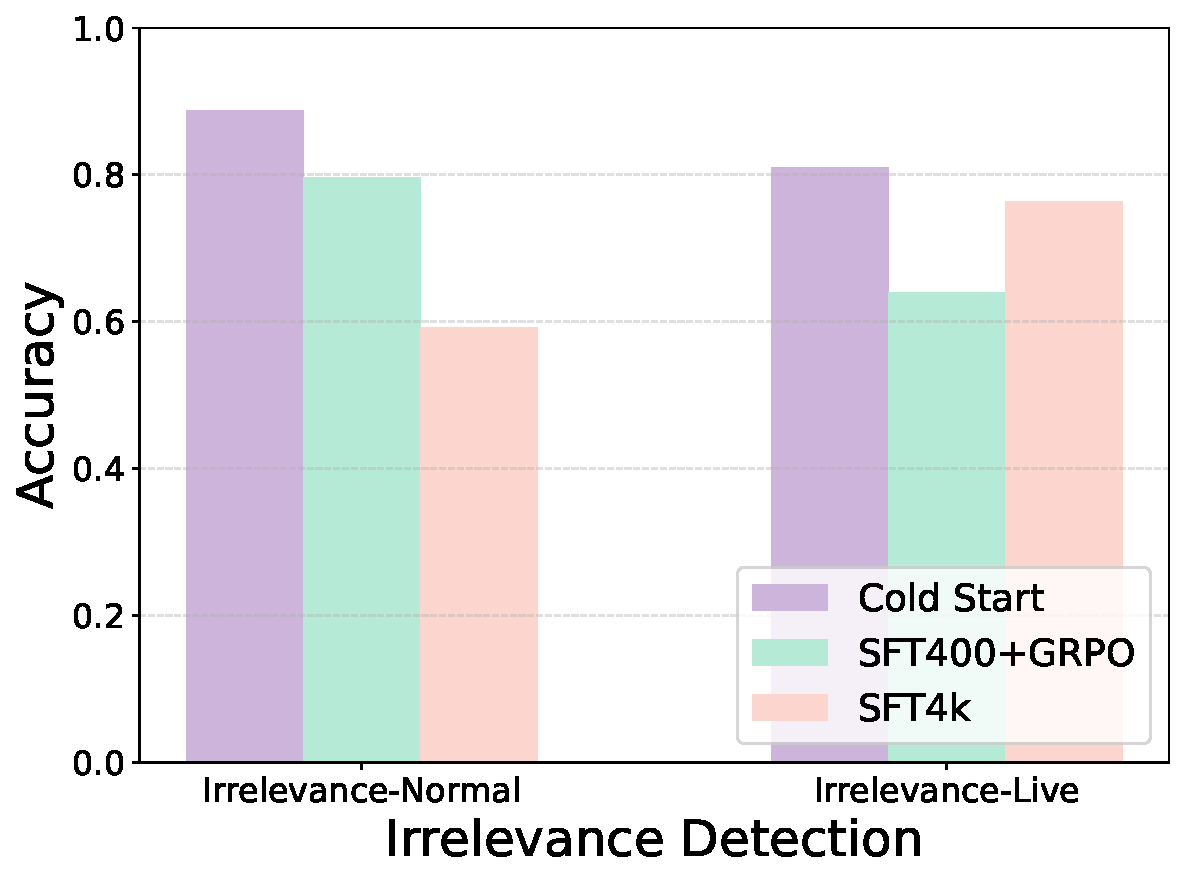
\includegraphics[width=0.469\linewidth]{figures/main_relevance.pdf}
    }
    \caption{Qwen2.5-3B-Instruct's performance across unfamiliar programming language scenarios (left) and novel relevance detection task goals (right), evaluated under different training settings.}
    \label{fig:main_generalization}
\end{figure}

\begin{table}[t]
\tiny
    \centering
    \begin{minipage}{0.5\textwidth}
        \centering

\begin{tabular}{l}
\toprule 
User: I would like to buy a movie ticket in San Jose at 11 o'clock in the night.\\
Tools Available:\\
\texttt{1. Movies\_1\_BuyMovieTickets(movie\_name, number\_of\_tickets, ...)}  \\
→ Buy tickets for a movie at a specific time and location.\\
\texttt{2. Movies\_1\_FindMovies(location, ...)}  \\
→ Search movies by location, genre, or format.\\
\texttt{3. Movies\_1\_GetTimesForMovie(movie\_name, location, ...)}  \\
→ Get showtimes for a movie on a specific date and location.\\
\midrule
\blue{<think>} The user wants to buy a movie ticket in San Jose at 11 PM. The available\\
tool, \texttt{Movies\_1\_BuyMovieTickets}, allows us to purchase movie tickets with the\\
required details such as movie name, number of tickets, show date, location, show time, \\
and show type. We need to find the movie name and the show date. However, the user \\
\green{did not specify the movie name or the show date}. We can infer the show date from the \\
current date, but we need to know the movie name to proceed with purchase. \blue{</think>} \\
\\
\purple{<response>} To assist in purchasing a movie ticket, \green{I need the name of the movie and} \\
\green{the specific date of the show}. Could you please provide this information? \purple{</response>} \\
\bottomrule
\end{tabular}

    \end{minipage}%
    \vspace{5pt}
    \begin{minipage}{0.5\textwidth}
        \centering

\begin{tabular}{l}
\toprule 
User: What is the slope of the line which is perpendicular to the line with the \\
equation y = 3x + 2?\\
Tools Available:\\
\texttt{1. find\_critical\_points(function, variable, range=[0.0, 3.4])}  \\
→ Find critical points of a function with respect to a variable, optionally \\
within a range.\\
\midrule
\blue{<think>} The problem is asking for the slope of a line that is perpendicular \\
to the line with the equation y = 3x + 2. The slope of the given line is 3. The slope \\
of a line that is perpendicular to another line is the negative reciprocal of the \\
original line's slope. So, the slope of the line perpendicular to y = 3x + 2 would be -1/3.\\
The given tool \texttt{find\_critical\_points} is \green{not relevant to finding the slope of a line and} \\
\green{cannot be used to solve this problem}. \blue{</think>} \\
\\
\purple{<response>} The slope of the line that is perpendicular to the line with the \\
equation y = 3x + 2 is \green{-1/3}. \purple{</response>} \\
\bottomrule
\end{tabular}

    \end{minipage}

    \label{tab:generalization_cases}
    \caption{Cases of Qwen2.5-3B-Instruct (GRPO Cold Start) generalizing to irrelevant tool detection goals.}
    
\end{table}

\paragraph{Generalization Studies.} We evaluate the generalization ability of our trained model in two challenging settings: unfamiliar scenarios and novel task goals (both from BFCL benchmark subset). Specifically, we test the model's performance in tool usage within unseen programming languages and its ability to detect irrelevant tools, neither of which were explicitly included during RL training or in the dataset. As shown in \Cref{fig:main_generalization}, Qwen2.5-3B-Instruct, when trained from scratch with our GRPO-based reward design, consistently achieves highest performance. Additionally, \Cref{tab:generalization_cases} presents two qualitative examples where the model proactively rejects inappropriate tool use—first by clarifying ambiguous intent, and second by opting to answer directly without tools. These behaviors reflect emergent proactivity and metacognition, enhancing efficiency, reducing hallucinations, and signaling foundational agentic intelligence.

\paragraph{Free-form Inference Effectiveness.} While our model is trained with a focus on tool call format and correctness, we further evaluate its ability to handle free-form tool use in a QA setting. Unlike the structured tool selection and application tasks, QA setting: (1) imposes no constraints on tool call parameters, and (2) evaluates only the final answer, making it a ``goal-oriented'' rather than a ``process-oriented'' task. This naturally introduces a multi-step interaction scenario.

Specifically, we use Bamboogle, a multi-hop QA dataset, to assess this capability. The model is equipped with a web search tool, and we report both the answer accuracy and the number of tool calls for all baselines and our approach. As shown in \Cref{tab:bamboogle-result-main}, our reward design achieves the highest performance, despite this setting not being explicitly seen during training. Notably, our cold start GRPO model surpasses others in accuracy without relying on excessive number of tool calls. This suggests that the model can flexibly invoke tools when needed, effectively leverage feedback, wisely and efficiently navigating toward the correct answer.


% \paragraph{Tool Use Behavior Analysis}


